\section{建模}\label{sec:models}

\subsection{横截面预测与无文本基准}

同一份 MPR 对全部行业提供同一个情绪分数。在含截距的单季横截面回归中，共同情绪与截距完全共线。用情绪给行业排序，需要先确定行业间的暴露差异。E4 沿用 Fama--MacBeth 的逐期横截面估计思路\cite{famaMacBeth1973}。设报告所属季度为 $q$，目标季度为 $t=q+1$，行业为 $i$，对数收益为 $r_{i,t}$。本文比较以下两个嵌套的模型设定：
\begin{equation}
  r_{i,t}=\alpha_t+\boldsymbol{b}_t^{\mathsf T}\boldsymbol{x}_{i,q}
     +\boldsymbol{d}_t^{\mathsf T}\boldsymbol{D}_i
     +\theta_t\bigl(z(S_q)\,z_q(B_{i,q})\bigr)+\varepsilon_{i,t}.
  \label{eq:fmb-with-text}
\end{equation}
无文本基准省去最后的交互项。$\boldsymbol{x}_{i,q}$ 包含报告期行业收益、报告期日收益年化波动率及截至发布日期用至多 120 个交易日估计的市场 beta，按当季行业截面标准化。$\boldsymbol{D}_i$ 为行业板块虚拟变量。$S_q$ 的标准化使用截至当期的扩展窗口。行业情绪暴露 $B_{i,q}$ 为截至报告期最近至多 20 个可配对季度中，行业同期收益对原始情绪分数的回归斜率，至少需 8 期，再按当期行业截面标准化，得到 $z_q(B_{i,q})$。式~\eqref{eq:fmb-with-text} 不另纳入暴露主效应，因为它与交互项在单季内共线。因而 $\theta_t$ 衡量该交互信号与收益的关系，无法单独识别情绪相对于一般行业暴露的边际效应。

E4 将 102 个目标季度依时间排序，2001Q2 至 2015Q4 为初始训练区间，2016Q1 至 2020Q4 为验证区间，2021Q1 至 2026Q3 为测试区间。每季单独估计系数，计算跨季均值及 Newey--West（NW）标准误，滞后阶为 2\cite{neweyWest1987}。样本外预测用该目标季之前的可拟合季度系数均值，随时间扩展并更新，已经结束的验证和测试季度可进入后续拟合。旧口径目标为报告期的下一季度，每个目标季均在报告发布前开始，平均早约 40.9 个日历日。下文将 E4 和 E6 的样本外结果作为对已实现季度收益的回溯比较。以完整的发布后收益且只用已实现历史训练标签的前瞻评价见第~\ref{sec:strict-timing}节。

排序指标 IC 是各季预测值与实际行业收益的 Spearman 秩相关，ICIR 是各季 IC 的均值与标准差之比。误差指标 MAE 是全部评估行业与季度的绝对预测误差均值。样本外 $R^2$ 的定义为
\begin{equation}
  R^2_{\mathrm{OOS}}=1-\frac{\sum_t\sum_i(r_{i,t}-\widehat r_{i,t})^2}
                {\sum_t\sum_i(r_{i,t}-\overline r_t)^2},
  \label{eq:oos-r2}
\end{equation}
其中 $\overline r_t$ 为当季评估截面事后实现收益的均值，用于刻画误差相对于行业分化程度的大小。直接评价文本增量时，另以共同评估样本上的无文本模型作为预测参照。

\begin{table}[htbp]
  \centering\small
  \caption{旧收益窗口下的测试期模型比较（E4、E6）}\label{tab:model-oos}
  \begin{tabular}{lrrrrr}
    \toprule
    模型 & 观测数 & 平均 IC & ICIR & $R^2_{\mathrm{OOS}}$ & MAE \\
    \midrule
    无文本（共同样本） & 677 & $-0.0384$ & $-0.1167$ & $-0.5621$ & 0.08558 \\
    NTUSD 简体 & 677 & $-0.0169$ & $-0.0504$ & $-0.6041$ & 0.08734 \\
    DLUT & 677 & $-0.0274$ & $-0.1005$ & $-1.2019$ & 0.10375 \\
    领域词典 & 677 & $-0.0970$ & $-0.3557$ & $-0.6124$ & 0.08746 \\
    LLM & 677 & 0.0733 & 0.2021 & $-0.6561$ & 0.09004 \\
    NTUSD 简体与 LLM & 677 & 0.0697 & 0.1966 & $-0.6066$ & 0.08804 \\
    \bottomrule
  \end{tabular}
  \par\smallskip
  \parbox{0.9\linewidth}{\footnotesize 注：测试区间共 23 季。无文本模型在 NTUSD 简体模型的有效预测行上重新计分。无文本模型使用全部 698 行时，平均 IC、$R^2_{\mathrm{OOS}}$ 和 MAE 分别为 $-0.0369$、$-0.5720$ 和 0.08530。数据取自 E4、E6 样本外指标表。}
\end{table}

表~\ref{tab:model-oos}中，主词典在测试期的平均 IC 较无文本基准高 0.0214，但两者均为负。其 $R^2_{\mathrm{OOS}}$ 更低，MAE 高约 2.05\%。验证期共同样本为 548 行，主词典的平均 IC 为 $-0.0129$，无文本为 $-0.0764$。主词典的 $R^2_{\mathrm{OOS}}$ 为 $-2.1728$，也低于无文本的 $-2.1106$。95 个可估计季度中，主词典交互系数均值为 $-0.0120$（NW $p=0.6200$），DLUT 的均值为 0.0465（NW $t=2.16$，原始 $p=0.0310$）。DLUT 的测试期误差大于主词典与无文本模型，且其系数显著性在第~\ref{sec:further}节的多重检验校正中消失。样本内系数的显著性与样本外预测表现给出了不同的判断。

\subsection{行业面板与固定效应}

行业固定效应吸收行业间不随时间变化的收益差别。E4 的行业固定效应模型纳入共同情绪、滞后行业收益、行业波动率、滚动市场 beta 以及按发布日对齐的宏观综合指标，标准误按行业聚类。主词典共同情绪系数为 0.00247（$t=0.64$，$N=2082$）。加入报告期固定效应后，共同情绪被吸收。另一设定保留行业与报告期固定效应，并加入情绪同收益、波动率和市场 beta 的交互项。主词典对应的三个交互项的聚类 $t$ 值依次为 $0.77$、$-0.39$ 和 $1.50$。这些估计表明，现有控制和固定效应下的情绪调节作用缺乏稳定证据。

\subsection{行业敏感度及其异质性}

E5 以市场模型、120 个交易日估计窗和 $[0,+1]$ 事件窗为主口径。对每个行业，将事件累计异常收益（CAR）对该期 NTUSD 简体原始情绪得分回归，所得斜率作为行业情绪敏感度。斜率在 $[-0.0643,0.0173]$ 之间，均值为 $-0.0281$，31 个行业中 3 个斜率为正。较晚起始的行业可匹配事件少，排序靠前或靠后都可能伴随较宽的区间。图~\ref{fig:industry-sensitivity}给出各行业的估计斜率与区间。

\begin{figure}[!htbp]
  \centering
  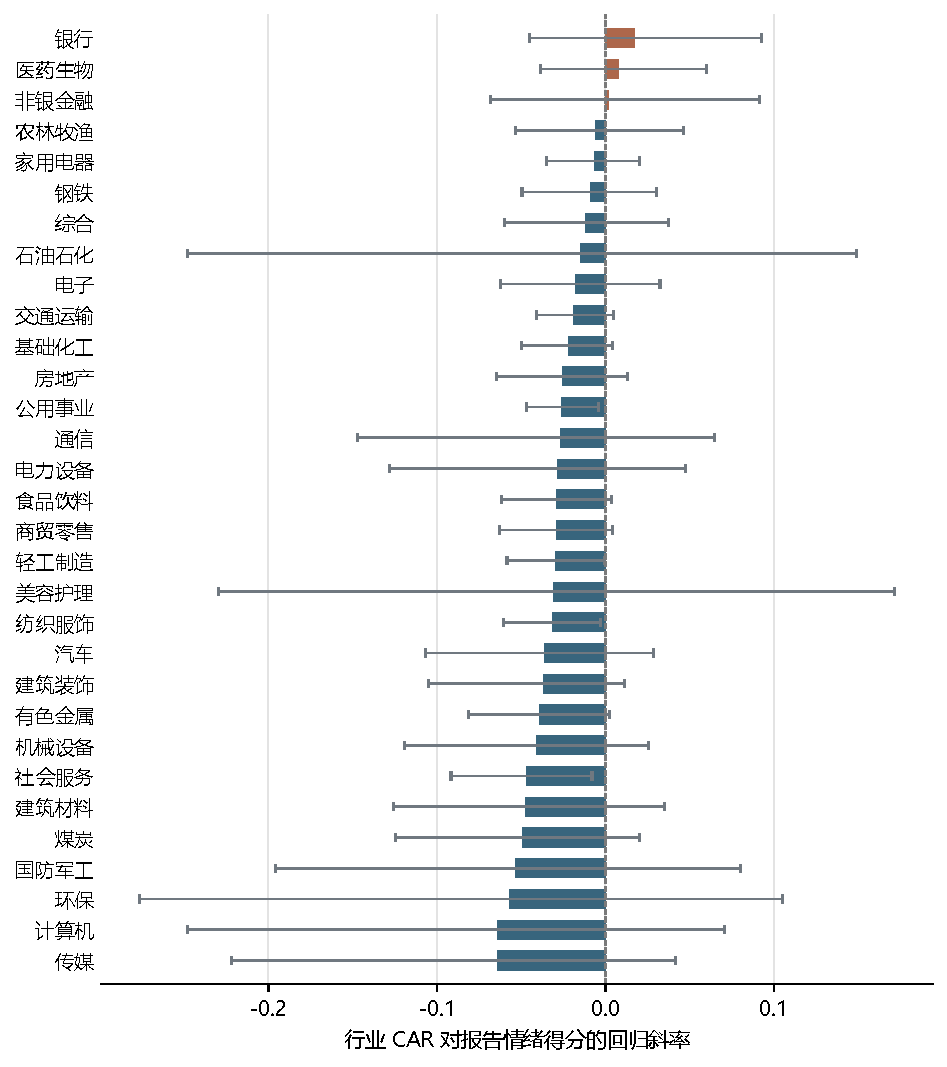
\includegraphics[width=0.96\linewidth,height=0.65\textheight,keepaspectratio]{fig19_heterogeneity.pdf}
  \caption{行业情绪敏感度与 95\% 置信区间（E5，按原始结果重排版）}\label{fig:industry-sensitivity}
\end{figure}

分析使用三项行业特征。利率敏感度由行业日超额收益对 10 年期国债收益率日变动的斜率度量，融资敏感度由行业月收益对社会融资规模累计同比变动的斜率度量。政策依赖指标将农林牧渔、银行、房地产、公用事业、建筑材料、建筑装饰及国防军工事先标为政策依赖行业。前两项在不同频率和覆盖长度下估计，第三项为定性代理。以行业估计斜率为因变量，在 31 个行业的横截面联合加入三项特征并使用 HC3 标准误，三项的原始 $p$ 值分别为 0.423、0.617 和 0.657。利率和融资敏感度分别单独入模时均达到 5\% 水平，但两者相关系数为 $-0.815$，联合估计难以区分相应关系。事件层面板另以 CAR 为因变量，保留行业固定效应并按事件聚类，逐一加入情绪与行业特征的交互项，三项的 $p$ 值均高于 0.10。

以 2014 年 2 月 21 日为界比较前后子样本，行业斜率的 Spearman 秩相关为 0.035（$p=0.897$），符号一致率为 38.7\%。由此，行业斜率存在数值差别，但联合横截面和事件层交互未为预设的三类特征提供稳定解释，跨时期的敏感行业排序也未复现。当前结果暂不支持 H3。

\subsection{大语言模型情绪及其增量}

E6 用大语言模型（LLM）对报告全文评分。固定模型别名 \texttt{qwen3.8-27b}、提示词 v1 和温度 0.0。分数取值 $[-1,1]$，综合政策立场、经济判断、风险、流动性和政策展望。提示词要求同时以结构化字段输出政策立场、各维度分数和原文依据，预测模型仅使用综合分数。103 期均得到可解析得分，其中部分报告在调整输出上限后获得有效响应。LLM 与 NTUSD 简体、DLUT、领域词典的 Pearson 相关分别为 0.213、0.326 和 0.042，说明评分差异需要结合下游结果和人工参照判断。

E6 沿用 E4 的面板、时间划分和信息集，用 LLM 分数与其滚动行业暴露构造交互项，比较词典模型、LLM 模型以及包含两个交互项的联合模型。测试期 LLM 的平均 IC 为 0.0733，词典为 $-0.0169$。LLM 的 IC 水平对零检验 $p=0.266$，与词典 IC 的点差不提供模型间显著改善的证据。LLM 的 $R^2_{\mathrm{OOS}}$ 低于词典，MAE 更大，验证期的排序指标也未同步改善。联合模型中 LLM 交互系数为 $-0.0272$（NW $p=0.684$），联合模型测试误差仍高于单独的 NTUSD 简体模型。评分差别与排序改善均不足以支持 H4 所要求的增量预测证据。

\subsection{多空组合及因子回归}

E7 把 E4 的样本外行业预测仅用作排序，持有期改为报告发布后的第一个完整自然季度。共形成 2016Q2 至 2026Q3 的 42 个组合季度，报告发布领先季初 35 至 57 个日历日。季初等权做多预测值最高的 5 个行业，等权做空最低的 5 个行业。多头和空头的绝对权重各为 100\%，按权重绝对变动的交易名义额计入单边 10 个基点的交易成本。无文本组合采用相同的行业池和持有期，另外保留同池行业等权、沪深 300 与随机分组用于参照。排序仍来自旧目标训练的模型，而且行业池沿用事后满足数据完整性要求的样本，组合结果用于描述排序在后移窗口内的表现。

图~\ref{fig:portfolio-equity}展示组合累计净值。计成本后，情绪多空组合的年化收益为 $-4.61\%$，夏普比率为 $-0.24$，最大回撤为 $-57.83\%$。无文本多空年化收益为 $-7.36\%$。分阶段看，情绪多空由验证期年化 $2.10\%$ 转为测试期 $-9.82\%$，测试期无文本为 $-8.59\%$。现有脚本以组合收益减去季度无风险收益为因变量，以中国三因子 CH3\cite{liuStambaughYuan2019}为自变量进行回归。因子覆盖不足的 2026Q2 和 2026Q3 从回归中剔除，保留 40 季。其截距季值经复利换算为年化 $2.65\%$（NW 滞后 1 阶，$t=0.46$）。该减无风险收益的约定与直接回归零成本多空价差的常见口径有别，不将其解释为标准零成本组合 alpha。收益仅反映设定的固定成本，组合实施还受融券供给、行业指数工具和市场冲击约束。

\paperfigure{fig18_portfolio_equity.pdf}{发布后完整季度的行业多空组合净值（E7，净成本与同池基准）}{fig:portfolio-equity}{0.96}

\subsection{模型结果小结}

回溯比较中，主词典模型在排序和误差指标上给出不同方向的变化。LLM 模型只提供局部排序改善，联合模型缺少显著增量。行业敏感度的排序和对行业特征的解释均缺乏跨设定支持。将组合收益移至发布后完整季度后，测试期也未观察到稳定的配置收益。下一章考察估计窗、文本来源及训练时点对这些结论的影响。

\section{进一步分析}\label{sec:further}

\subsection{事件窗、模型设定与多重检验}

E8 在事件模型和季度预测中改变词典、基准指数、窗口长度、样本切点、情绪编码、特征滞后及缩尾规则。49 个设定中，事件设定 23 个，旧收益窗口和时点修正窗口的预测设定各 13 个。39 个达到计算和最低样本要求，10 个在分组样本量、模型矩阵秩或固定测试期覆盖方面受限。事件对照按同一发行期与行业的交集比较，并在事件内等权汇总 CAR。季度预测对照在共同面板内重估，并按共同预测键计分。因此，使用中证全指后样本起点后移造成的差异，与同样本基准变化引起的差异分别记录。

事件比较用 $[0,+5]$ 作展示锚点，其他三个窗口同时列入检验。市场模型中，主词典的四个窗口下高减低 CAR 点估计同为负。$[0,+1]$ 的差为 $-0.609$ 个百分点（原始 $p=0.0113$），校正后的 $p$ 值为 0.2605。改用均值调整模型时，展示窗高减低差值转为正，原始 $p=0.485$。从估计窗中剔除与历史报告 $[0,+10]$ 窗口重叠的交易日后，差值为 $-0.574$ 个百分点（$p=0.247$）。这项处理针对估计窗重叠，同期市场消息仍有可能混入报告发布附近的收益。

事件主效应、旧口径预测系数、严格时点预测系数分别形成三个检验族，以 Benjamini--Hochberg（BH）与 Holm 法报告调整后的 $p$ 值\cite{benjaminiHochberg1995,holm1979}。原始 $p<0.05$ 的主效应共 3 项，两种调整后均无一项达到 5\% 水平。全样本平均 CAR 另列为次要检验族。不同设定重复使用相同报告与行业，BH 结果按探索性指标解释，Holm 提供对检验依赖结构要求较弱的校正。全部稳健性设定共记录 19,876 条底层失败或受限条目，其中部分条目对应多个行业或同一观测的不同设定。其数目不能解释为独立样本量。

\subsection{严格时点下的预测复核}\label{sec:strict-timing}

E8 将预测目标改为发布后的首个完整季度，并重估文本模型和无文本模型。模型以报告发布日期为预测原点，只用在该日期前已结束的历史收益季度更新系数，至少需 8 个可用历史拟合季度。旧口径的 2,274 个行业与季度观测均含发布前收益。修正后获得 2,243 个基础观测和 101 期报告，旧口径最后纳入的 2026Q2 报告对应的发布后完整季度落在观察期外。严格设定的预测记录均通过发布日及标签实现时点约束检查。已归档行情的行业分类、覆盖和事后补齐规则仍限制严格时点样本的解释。

\begin{table}[htbp]
  \centering\small
  \caption{发布后首个完整季度的配对测试结果（E8）}\label{tab:strict-oos}
  \begin{tabular}{lrrrr}
    \toprule
    模型 & 观测数 & 平均 IC & $R^2_{\mathrm{OOS}}$ & MAE \\
    \midrule
    无文本 & 674 & 0.0401 & $-0.5628$ & 0.08605 \\
    NTUSD 简体 & 674 & $-0.0074$ & $-0.9039$ & 0.09567 \\
    文本模型减无文本模型 & & $-0.0475$ & $-0.3410$ & 0.00962 \\
    \bottomrule
  \end{tabular}
  \par\smallskip
  \parbox{0.88\linewidth}{\footnotesize 注：两模型在共同面板上拟合，测试期均为 2021Q1 至 2026Q3，共 23 季。来源为 E8 严格时点参考设定的配对统计。}
\end{table}

严格时点结果见表~\ref{tab:strict-oos}。主词典在平均 IC、$R^2_{\mathrm{OOS}}$ 与 MAE 上均弱于无文本参照，交互系数均值为 $-0.0330$（NW 原始 $p=0.184$）。旧窗口下，NTUSD 简体与 DLUT 等权组合的个别样本外指标相对无文本模型略有改善，时点修正后该组合的增量 $R^2_{\mathrm{OOS}}$ 转为负。两套评估共同表明 H2 缺少稳定支持，其中严格时点口径只评价词典特征。LLM 特征仍需按同样的时点要求另行验证。

\subsection{LLM 敏感性与失败归因}

E9 冻结原始响应，在同一批 E6 响应上重放严格解析、E6 宽松解析及括号规范化三种审计规则，103 期均得到一致得分。配置比较使用新版逐响应审计与汇总表。按 E6 宽松解析，同一较早提示词在温度 0.0 下取得 91 期有效分数，提高至 0.7 后只有 31 期有效。高温设置的 67 次请求受 HTTP 429 限流，返回的 36 份中另有 5 份在输出触顶后未通过 JSON 解析。最简提示词在温度 0.7 的 103 次请求全部受限流，缺少可用于归因的模型响应。仅比较同一提示词在两种温度下共同有效的响应时，旧版提示词的分数 Pearson 相关约为 0.988。现有记录能量化输出可用性，温度对分数的独立作用还受共同样本选择影响。

跨模型比较原计划覆盖 39 期，归档请求清单每种别名覆盖 24 期。\texttt{gpt-4o} 的 24 期均可用，但可计算模型指标的验证期只有 2 季（平均 IC 为 0.322），测试期也只有 6 季（$-0.0374$）。\texttt{deepseek-v4-flash} 有效输出 17 期，\texttt{glm-5.3} 的请求全部受限流。模型比较样本稀疏，模型别名未绑定可核实的权重版本，且预测口径沿用 E6 的回溯窗口。这些条件限制了对提示词、模型和温度的横向比较。

\subsection{误差、异常与推断边界}

E10 对冻结输入作只读检查，记录 1,002 条复核条目。其中，521 条为市场交易日缺失或行情覆盖限制，287 条为预测残差异常，33 条为低词典覆盖抽检，29 条为 LLM 变体失败。异常残差按绝对值超过四分位距上栅栏判定。E8 严格时点的文本和无文本预测中，共有 57 条残差异常（1,348 条模型预测记录），异常组与其余组的平均绝对残差分别为 0.3274 和 0.0804。不同模型可能在同一行业季度同时出现异常，数量用于定位误差来源。另有 15 条人工评分待办来自 E10 生成时的快照。其后评分表已填入分数，评分人身份与独立重复评分的证据仍待补齐。

本文所用的解释变量来自季度报告中的共同信息，时间维度的有效观察数远少于行业与季度面板的行数。报告文字可能在同一文本中同时表达当前经济风险和未来宽松意图，单一情绪得分难以区分两者。行业敏感度还受行业历史覆盖、代理变量共线性、极端收益和正常收益模型选择制约。事件日后短窗与严格季度预测回答不同时间尺度的问题。现有证据在两种时间尺度上均不足以支撑稳定的正向收益关系，但仍容许不同文本维度、不同政策背景或不同观察频率下存在更局部的关系。
